\section{Opgave 1 - MeeMoo state machine}
\begin{enumerate}
	\item[1)]
	Vi har anvendt et Moore-template fra Quartus til at udforme nedenstående VHDL-kode for programmet:
	
\begin{lstlisting}[caption={VHDL koden for kodelås},label={lst:code_lock}]
library ieee;
use ieee.std_logic_1164.all;
use ieee.numeric_std.all;

entity code_lock is
port ( clk, reset, enter : in std_logic;
code : in std_logic_vector(3 downto 0);
lock : out std_logic;
state_led : out std_logic_vector(2 downto 0));
end code_lock;

architecture rtl of code_lock is

-- Build an enumerated type for the state machine
type state_type is (idle, code1acc, code2acc, wrong_code, perm_lock, unlocked);

-- Register to hold the current state
signal state   : state_type;
signal err_cnt : std_logic_vector(1 downto 0);
signal enter_last : std_logic;
signal code1, code2, code3 : std_logic_vector(3 downto 0);

begin

-- Logic to advance to the next state
state_reg: process (clk, reset)
begin
if reset = '0' then
err_cnt <= "00";
state <= idle;
elsif (rising_edge(clk)) then
enter_last <= enter;
case state is

when wrong_code=>
err_cnt <= std_logic_vector(unsigned(err_cnt) + 1);
if err_cnt >= "10" then
state <= perm_lock;
else
state <= idle;
end if;

when perm_lock =>
state <= perm_lock;

when idle =>
lock <= '0';
if enter_last = '1' and enter = '0' then
if code = code1 then
state <= code1acc;
else 
state <= wrong_code;
end if;
else
state <= idle;
end if;

when code1acc =>
if enter_last = '1' and enter = '0' then
if code = code2 then
state <= code2acc;
else 
state <= wrong_code;
end if;
else
state <= code1acc;
end if;

when code2acc =>
if enter_last = '1' and enter = '0' then
if code = code3 then
state <= unlocked;
else 
state <= wrong_code;
end if;
else
state <= code2acc;
end if;

when unlocked =>
lock <= '1';
if enter_last = '1' and enter = '0' then
state <= idle;
else
state <= unlocked;
end if;
end case;
end if;
end process;

-- Output depends solely on the current state
ledoutput: process (state)
begin
case state is
when idle =>
state_led <= "001";
code1 <= "0001";
when code1acc =>
state_led <= "011";
code2 <= "0010";
when code2acc =>
state_led <= "111";
code3 <= "0011";
when others =>
state_led <= "000";
end case;
end process;

end rtl;



\end{lstlisting}

Vi har pin-assignet på De2-boardet, således at koden kan skrives på SW[3..0], enter-knap ligger på KEY[0] og reset-knap på KEY[3]. Outputs ligger henholdsvis på LEDG[7], som viser om systemet er låst eller oplåst og LEDR[1:0], som viser hvilken state vi er i. 

\begin{figure}[h]
	\centering
	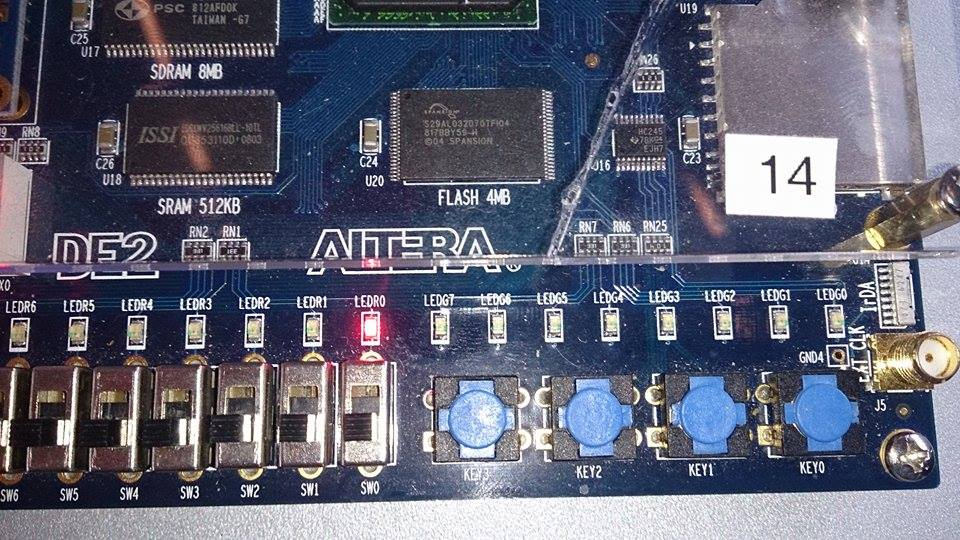
\includegraphics[scale=0.45]{pictures/Oevelse7/opg2/StateIdle.JPG}
	\caption{State idle}
	\label{fig:}
\end{figure}
		
\begin{figure}[h]
	\centering
	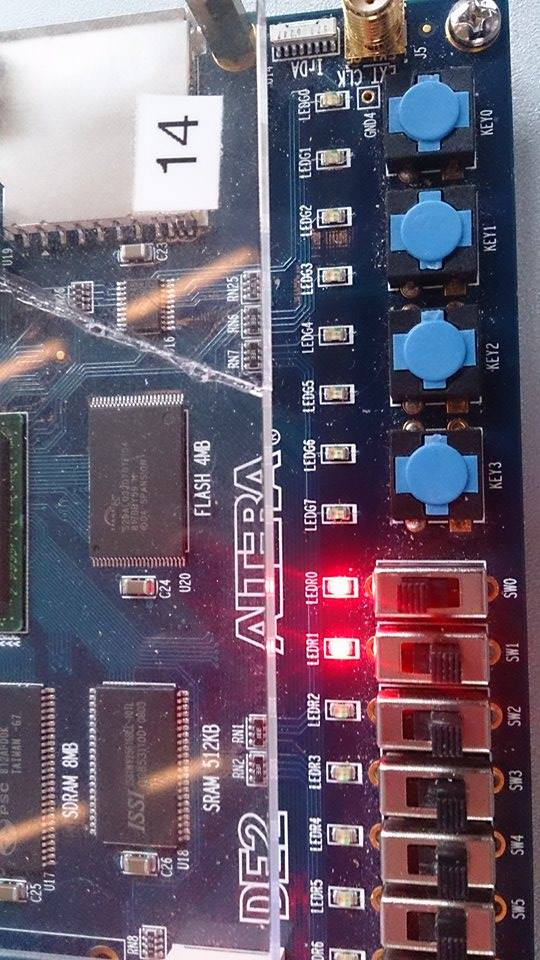
\includegraphics[scale=0.45]{pictures/Oevelse7/opg2/StateTwo.JPG}
	\caption{State two - code 1 accepted}
	\label{fig:}
\end{figure}

\begin{figure}[h]
	\centering
	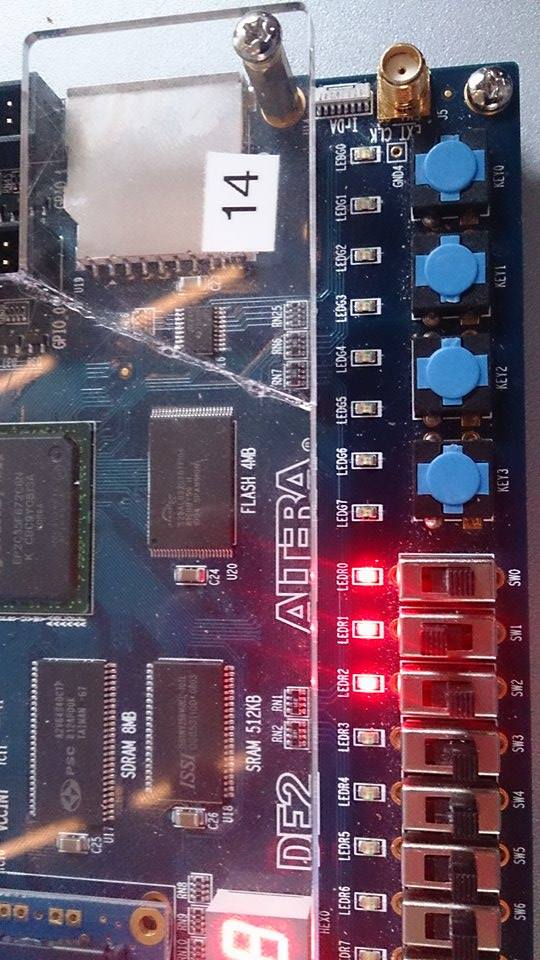
\includegraphics[scale=0.45]{pictures/Oevelse7/opg2/StateThree.JPG}
	\caption{State three - code 2 accepted}
	\label{fig:}
\end{figure}

\begin{figure}[h]
	\centering
	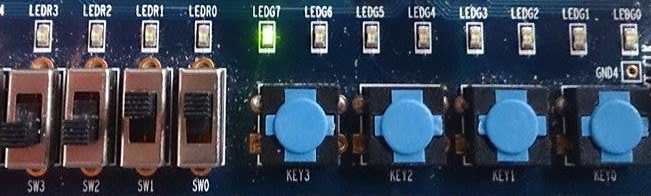
\includegraphics[scale=0.45]{pictures/Oevelse7/opg2/StateUnlocked.JPG}
	\caption{State unlocked - code 3 accepted}
	\label{fig:}
\end{figure}

\begin{figure}[h]
	\centering
	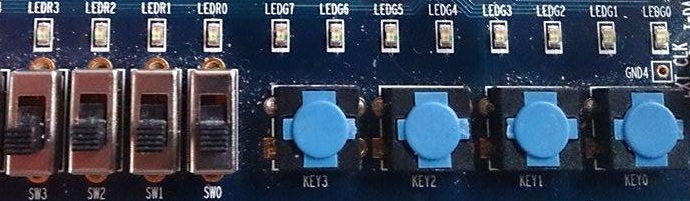
\includegraphics[scale=0.45]{pictures/Oevelse7/opg2/StatePermLocked.JPG}
	\caption{State permanently locked}
	\label{fig:}
\end{figure}

\end{enumerate}
	